% Asset ID: AS1VectorsTikZ-006
% Asset type: TikZ diagram
% Suggested file: tikz/AS1VectorsTikZ-006_unit_vector.tex
% Source: CCEA AS1-VEC-LO002; Phase 1 Core Theory 4
% Related lesson section: Unit vectors; Worked Example 4
% Purpose: Show that a unit vector is found by dividing a vector by its magnitude.
% Boundary note: 2D vectors only.

\documentclass[tikz,border=8pt]{standalone}
\usepackage{amsmath}
\usetikzlibrary{arrows.meta, positioning}
\begin{document}
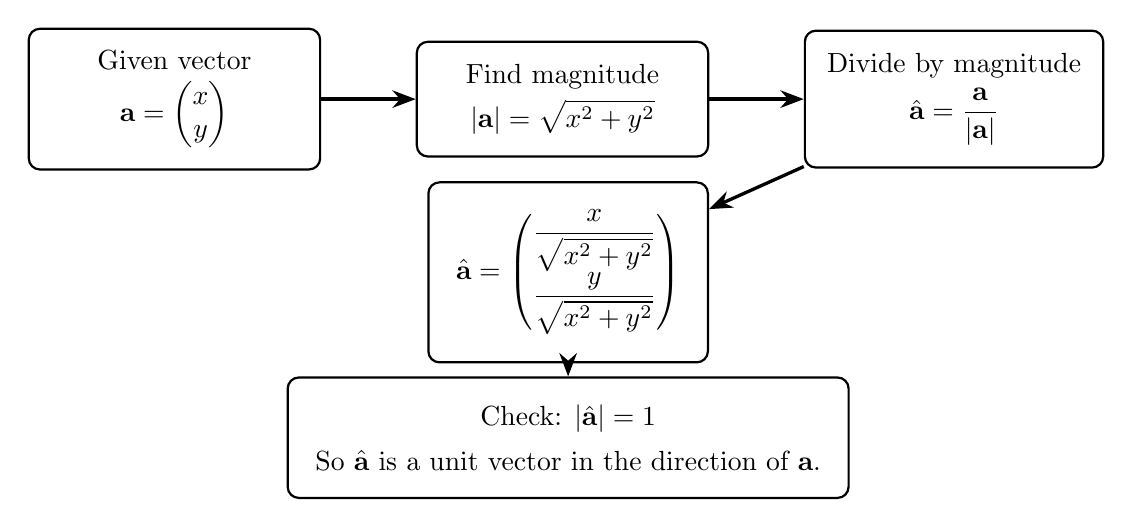
\begin{tikzpicture}[>=Stealth,box/.style={draw, rounded corners, thick, align=center, minimum width=3.7cm, minimum height=1.2cm, inner sep=8pt},arrow/.style={->, very thick},formula/.style={draw, rounded corners, thick, align=center, inner sep=10pt}]
\node[box] (start) at (0,0) {Given vector\\[3pt] $\displaystyle \mathbf{a}=\begin{pmatrix}x\\y\end{pmatrix}$};
\node[box, right=1.2cm of start] (mag) {Find magnitude\\[3pt] $\displaystyle |\mathbf{a}|=\sqrt{x^2+y^2}$};
\node[box, right=1.2cm of mag] (divide) {Divide by magnitude\\[3pt] $\displaystyle \hat{\mathbf{a}}=\frac{\mathbf{a}}{|\mathbf{a}|}$};
\draw[arrow] (start) -- (mag); \draw[arrow] (mag) -- (divide);
\node[formula] (result) at (5,-2.2) {$\displaystyle \hat{\mathbf{a}}=\begin{pmatrix}\dfrac{x}{\sqrt{x^2+y^2}}\\[8pt]\dfrac{y}{\sqrt{x^2+y^2}}\end{pmatrix}$};
\node[formula] (check) at (5,-4.3) {Check: $\displaystyle |\hat{\mathbf{a}}|=1$\\[4pt] So $\hat{\mathbf{a}}$ is a unit vector in the direction of $\mathbf{a}$.};
\draw[arrow] (divide) -- (result); \draw[arrow] (result) -- (check);
\end{tikzpicture}
\end{document}
